%%%%%%%%%%%%%%%%%%%%%%%%%%%%%%%%%%%%%%%%%%%%%%%%%%%%%%%%%%%%%%%%%%%%%%%%
% Preamble
%%%%%%%%%%%%%%%%%%%%%%%%%%%%%%%%%%%%%%%%%%%%%%%%%%%%%%%%%%%%%%%%%%%%%%%%
\documentclass[11pt]{article}
%
% Packages and other includes
% Pagination
\usepackage[letterpaper, margin=1in]{geometry}
\usepackage{emptypage}
%
% Fonts
\usepackage[T1]{fontenc} % best for Western European languages
\usepackage{lmodern} % Latin Modern instead of CM
\usepackage{textcomp} % required to get special symbols
%
% Math
\usepackage{amsmath, amssymb}
\usepackage{braket}
%
% Graphics, floats, tables
\usepackage{graphicx, color, float, array}
%
% Hyperlinks
\usepackage{hyperref}
%
%
% Definitions and settings
% Paragraph indent and spacing
\setlength{\parskip}{0.4\baselineskip}
\setlength{\parindent}{0in}
%
%
% Title, authors, date
\title{\textbf{Worksheet 1}}
\date{\vspace{-2em}\today}
%
%
%%%%%%%%%%%%%%%%%%%%%%%%%%%%%%%%%%%%%%%%%%%%%%%%%%%%%%%%%%%%%%%%%%%%%%%%
% Main document
%%%%%%%%%%%%%%%%%%%%%%%%%%%%%%%%%%%%%%%%%%%%%%%%%%%%%%%%%%%%%%%%%%%%%%%%
%

\begin{document}

\maketitle

Weekly homework assignments are posted approximately one week prior to the
due date. Collaborations are encouraged and students must report all collaborators
in writing on each assignment. All external sources (websites, books) must be
properly cited. Additional problems are listed at the end of each assignment.
This week's assignment is due \textit{Tuesday, Jan 11th at 10:00am.}

\textbf{Zeroth Law of Thermodynamics}

1. (2 pts) Suppose a system is in thermal equilibrium with a heat bath. If the temperature
of the heat bath increases, describe in words and/or illustrations what happens to
the temperature of the system.

% The temperature of the system increases since the heat bath increases.
% 
%\begin{center}
%  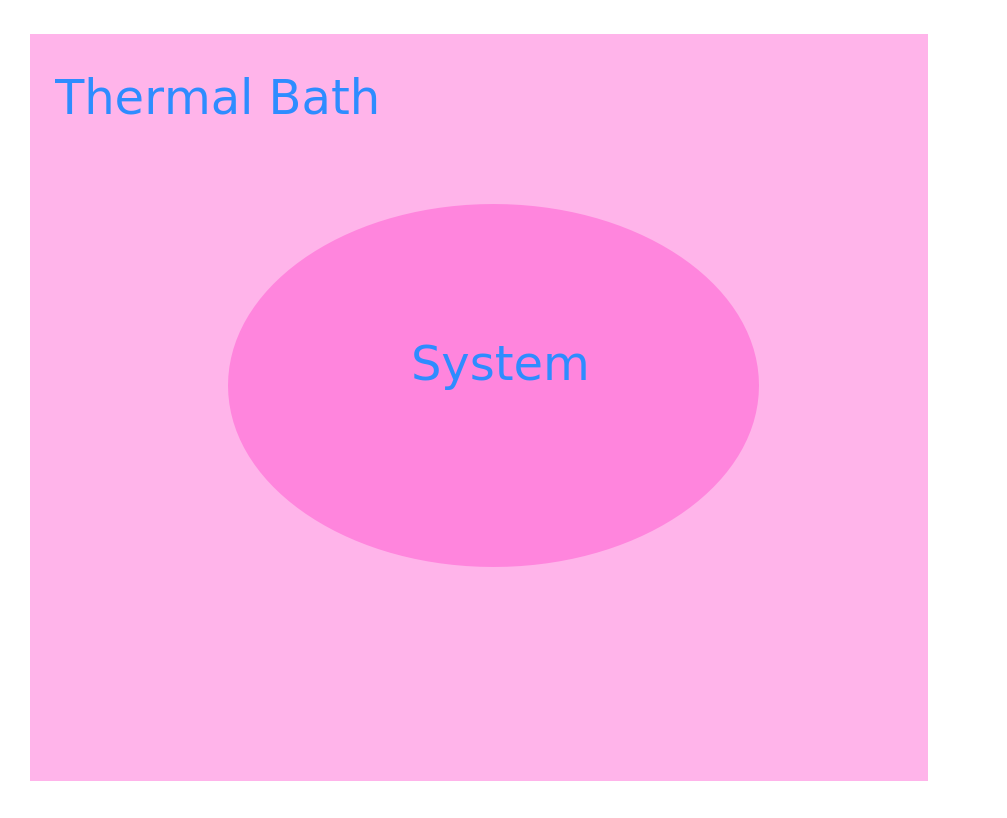
\includegraphics[scale=0.3]{therm_equil.png}
%\end{center}

\vspace{2in}

2. (2 pts) Consider two isolated systems illustrated below. One system (left) is at $100^\circ\text{C}$
and the other (right) is at room temperature of $20^\circ\text{C}$. The isolated systems are allowed
to come into contact reaching thermal equilibrium and without losing energy to the surrounding.
What is the final temperature? Describe in words and/or illustrations what happened.

\begin{center}
  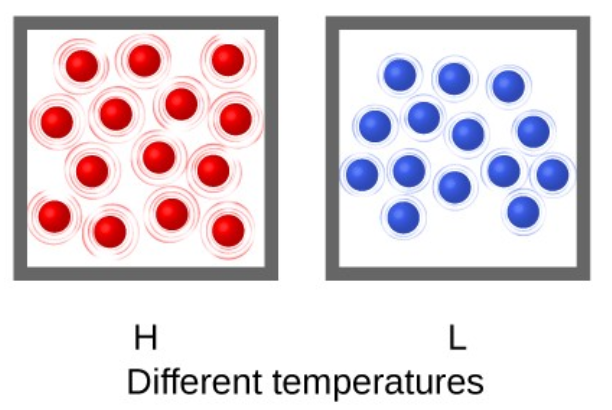
\includegraphics[scale=0.25]{isolated_sys.png}
\end{center}

% 60C is the final temperature; heat move from hot to cold

\vspace{2.5in}

\textbf{Ideal Gas Law}

3. (4 pts) \textbf{Gay-Lussac's Law}: A $250.$ mL aerosol can at $25.0^\circ\text{C}$ and $1.10$ atm was
thrown into an incinerator. When the temperature in the can reached $712^\circ\text{C}$, the
can exploded. What was the pressure in the can just before it exploded, assuming it reached
the maximum pressure possible at that temperature in $^\circ\text{C}$? Report to 3 significant figures.

% P/T = nR/V since P and V are not constant
% 3.63 atm

\vspace{2.5in}

4. (4 pts) The Victor Meyer's method (illustrated below) is used to measure molecular mass. This
is accomplished by vaporizing a known mass of a volatile solid or liquid and measuring
the volume of air displaced over water. Suppose 0.200g of a white crystalline solid sample is
vaporized. The gas is collected over water at 1.00 atm and $25.0^\circ\text{C}$ and displaces
51.8 mL of air. What is the molar mass of the sample? Report to 3 significant figures.

\begin{center}
  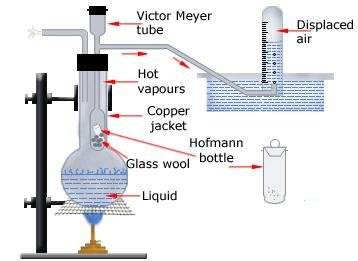
\includegraphics[scale=0.55]{meyers.jpeg}
\end{center}

% n = PV/RT
% computed molar mass is 94.5 g/mol
% 
%phenol 94.11 g/mol

\vfill
\textbf{Additional Problems:} Ch. 10 - odd problems 25 - 57, 83, 85, and 89.

%1. Review: Balancing chemical equations.
%\begin{enumerate}
%\item[a)] \,\,\, C$_6$H$_{12}$O$_6$(s) + \,\,\, O$_2$(g) $\rightarrow$ \,\,\, CO$_2$(g) + \,\,\, O$_2$(g)
%  %combustion reaction
%\item[b)] \,\,\, C$_2$H$_6$(g) + \,\,\, O$_2$(g) $\rightarrow$ \,\,\, CO$_2$(g) + \,\,\, H$_2$O
%\item[c)] \,\,\, CuS(s) + \,\,\, HNO$_3$(aq) $\rightarrow$ \,\,\, CuSO$_4$(aq) + \,\,\, NO$_2$(g)
%  %extracting copper from the mineral covellite (CuS); Oxidation-reduction reaction
%\end{enumerate}

%1. Define state function. Determine whether the following are state functions:
%\begin{enumerate}
%\item[a)] $q + w$ % yes
%\item[b)] $\Delta H$ % yes
%\item[c)] $q$ % no
%\item[d)] Volume % no
%\end{enumerate}

%2. Which statement is true of the internal energy of a system and its
%surroundings during an energy exchange with a positive $\Delta E_\text{sys}$?
%\begin{enumerate}
%\item[a)] The internal energy of the system increases, and the internal
%  energy of the surroundings decreases.
%\item[b)] The internal energy of both the system and the surroundings
%  increases.
%\item[c)] The internal energy of both the system and the surroundings
%  decreases.
%\item[d)] The internal energy of the system decreases, and the internal
%  energy of the surroundings increases.
%\end{enumerate}
% a)

%3. A system absorbs 196 kJ of heat, and the surroundings do 117 kJ
%of work on the system. What is the change in internal energy of
%the system?
% 313 kJ

%4. The air within a piston equipped with a cylinder absorbs 565 J of 
%heat and expands from an initial volume of 0.10 L to a final volume of
% 0.85 L against an external pressure of 1.0 atm. What is the change in
% internal energy of the air within the piston?
% 489 J
\end{document}
